\chapter{Primitive content and the cost of clearing}
\label{chap:primitive-content}

\section{Three integers with different jobs}

The packet coefficients are rational before denominators are cleared. Their common divisor depends on the chosen clearing factor. The rational approximation and its primitive integer linear form do not. This distinction is the central arithmetic issue in the five historical gcd calculations.

Fix integers $n,m\geq0$, and write
\begin{equation}
 U=\sum_{i=0}^{m}\binom miT_{n+i},\qquad
 V=\sum_{i=0}^{m}\binom mi16^{n+i}v_{n+i}.
 \label{eq:primitive-UV}
\end{equation}
These are fixed-pair aliases $U=S_{n,m}$ and $V=H_{n,m}$ for the packets defined earlier, not the integral coefficients of a different source normalization. Here $T_k=16^ku_k$ is a positive integer. Consequently $U$ is a positive integer. Write $V=N/D$ in lowest terms, with $D>0$ and $\gcd(N,D)=1$. In the exceptional case $V=0$, the same convention sets $N=0,D=1$. Set
\begin{equation}
 \ell=2(n+m),\qquad L_\ell=\operatorname{lcm}(1,\ldots,\ell),
 \qquad Q=8L_\ell^2,
 \label{eq:Q-clearance}
\end{equation}
with $L_0=1$.

The source arithmetic ensures $QV\in\Z$. Indeed, the strong coefficient theorem gives $4\cdot16^kL_{2k}^2v_k\in\Z$, and $L_{2k}\mid L_\ell$ for $k\leq n+m$. The weaker factor $8$ in $Q$ therefore clears every summand in \eqref{eq:primitive-UV}. Since $V=N/D$ is reduced, this proves $D\mid Q$. The factor $Q$ is a convenient universal choice. The factor $D$ is the actual least denominator of this particular rational packet.

The historical cleared coefficients are
\begin{equation}
 A=(-1)^nQU,\qquad B=(-1)^nQV,
 \qquad g=\gcd(|A|,|B|).
 \label{eq:cleared-pair}
\end{equation}
The sign changes neither the gcd nor the approximation $B/A=V/U$. Finally put
\begin{equation}
 h=\gcd(DU,N).
 \label{eq:minimal-content}
\end{equation}
This is the content of the minimally cleared pair. It must not be confused with $g$. The three quantities $Q$, $D$, and $h$ record, respectively, the chosen clearing factor, the actual packet denominator, and the common content left after minimal clearing.

\section{An exact decomposition}

\begin{proposition}[Redundant clearance and primitive content]
\label{prop:content-decomposition}
For the coefficients above,
\begin{equation}
 h=\gcd(U,N),\qquad
 g=\frac QD\,h.
 \label{eq:gcd-decomposition}
\end{equation}
The reduced rational approximation and primitive coefficients are
\begin{equation}
 \frac VU=\frac{N/h}{DU/h},\qquad
 \frac Ag=(-1)^n\frac{DU}{h},\qquad
 \frac Bg=(-1)^n\frac Nh.
 \label{eq:primitive-pair}
\end{equation}
In particular the positive reduced denominator is $q=DU/h$.
\end{proposition}

\begin{proof}
If $N=0$, the reduced convention gives $D=1$. Since $U>0$, one has $h=U$, $g=QU$, and the unsigned primitive pair is $(1,0)$. All the stated identities follow directly in this case. Assume now $N\ne0$. Since $\gcd(D,N)=1$, multiplication of $U$ by $D$ adds no prime factor that can divide $N$. Prime by prime, $\min\{v_p(DU),v_p(|N|)\}=\min\{v_p(U),v_p(|N|)\}$. This proves the first equality. Next write $Q=cD$, where $c$ is a positive integer. The unsigned cleared pair is $(cDU,cN)$, so its gcd is $c\gcd(DU,N)=ch$. Dividing both coefficients by this gcd proves the remaining identities. The pair $(DU/h,N/h)$ is coprime by the definition of $h$, which proves the claim about the reduced denominator.
\end{proof}

The decomposition contains no asymptotic assumption. It holds at each individual pair $(n,m)$. Its usefulness is that it assigns every common factor to a precise source. A large value of $g$ can be caused by a large value of $Q/D$, even when $h$ is small. Such a factor reflects an unnecessarily generous initial clearing choice. It is not additional content in the minimally cleared pair.

For the historical normalization of the integral filter,
\begin{equation}
 \widetilde J_{n,m}
 =8(-1)^n16^{-n}(UG-V).
 \label{eq:primitive-filter-normalization}
\end{equation}
Thus the primitive integer linear form is
\begin{align}
 \Lambda_{n,m}
 &=\frac AgG-\frac Bg
 =(-1)^n\frac D h(UG-V)\notag\\
 &=\frac{16^nL_\ell^2}{g}\,\widetilde J_{n,m}.
 \label{eq:primitive-error}
\end{align}
Every normalization factor in this formula matters. In particular, the $8$ in $Q$ cancels the $8$ in \eqref{eq:primitive-filter-normalization}. The right side is a real expression for a linear form with integer coefficients. Its absolute value is independent of whether the signs are carried in $A,B$ or in the filter.

\section{Scaling does not manufacture an improvement}

\begin{proposition}[Invariance under additional clearing]
\label{prop:scale-invariance}
If an integer pair $(A,B)$ is replaced by $(cA,cB)$ for an integer $c>0$, then its primitive pair and primitive linear form remain unchanged. More generally, any integer clearing factor $Q'$ divisible by $D$ gives the same unsigned primitive pair $(DU/h,N/h)$.
\end{proposition}

\begin{proof}
The equality $\gcd(cA,cB)=c\gcd(A,B)$ proves the first statement. For the second, apply Proposition~\ref{prop:content-decomposition} with $Q'$ in place of $Q$. The factor $Q'/D$ cancels exactly on division by the new gcd.
\end{proof}

This observation blocks a tempting but invalid arithmetic argument. One can make the cleared gcd arbitrarily large by multiplying both coefficients by a large integer. Doing so also enlarges the error by precisely the same factor. After reduction there is no change. Any proposed gain must be measured in the primitive form \eqref{eq:primitive-error}, or equivalently in the reduced denominator $q=DU/h$.

An elementary example makes the cancellation visible. Take $U=12$ and $V=10/9$. The minimally cleared pair is $(108,10)$ and has gcd $2$. Its primitive pair is $(54,5)$. Clearing instead with $Q=90$ gives $(1080,100)$ and gcd $20$. The apparent tenfold increase in gcd is exactly the tenfold excess in the clearing factor. Both pairs reduce to $(54,5)$ and both represent the approximation $5/54$.

There is still a legitimate role for a redundant clearing factor. It can make a universal theorem easy to state and a program easy to reproduce. The correction is accounting, not a ban on convenient denominators. A calculation with $Q$ is valid when the reduction by $g$ is kept in the same formula. A calculation that counts $g$ as a gain while ignoring the corresponding size of $Q$ is not valid.

\section{The five recovered rows}

The historical script recorded five pairs near the slope used in Eskandari's filter. The fresh exact run reproduces their gcds and factorizations. An independent rational calculation also extracts $D$, $Q/D$, and $h$. The resulting decomposition is as follows.

\begin{table}[htbp]
\centering\small
\begin{tabular}{@{}rrrrr@{}}
\toprule
$(n,m)$ & $Q/D$ & $h$ & $g$ & $v_2(g)$\\
\midrule
$(20,66)$ & $1\,703\,936$ & $8$ & $13\,631\,488$ & $20$\\
$(30,100)$ & $129\,499\,136$ & $4$ & $517\,996\,544$ & $21$\\
$(50,166)$ & $2\,779\,250\,688$ & $8$ & $22\,234\,005\,504$ & $22$\\
$(70,232)$ & $5\,257\,560\,064$ & $64$ & $336\,483\,844\,096$ & $27$\\
$(100,332)$ & $1\,084\,227\,584$ & $8$ & $8\,673\,820\,672$ & $24$\\
\bottomrule
\end{tabular}
\caption{Exact content decomposition at the five historical pairs. These are finite values, not an asymptotic law.}
\label{tab:content-five}
\end{table}

The factorizations of the cleared gcds are
\begin{align*}
13\,631\,488&=2^{20}\cdot13,\\
517\,996\,544&=2^{21}\cdot13\cdot19,\\
22\,234\,005\,504&=2^{22}\cdot3^2\cdot19\cdot31,\\
336\,483\,844\,096&=2^{27}\cdot23\cdot109,\\
8\,673\,820\,672&=2^{24}\cdot11\cdot47.
\end{align*}
For these rows the minimally cleared gcd has only the powers of $2$ displayed in $h$. All odd factors in the listed cleared gcds belong to $Q/D$. That conclusion is specific to these five pairs. It does not establish that odd primitive content is always absent.

The first row illustrates the exact check without printing its very large numerator and denominator. The independently reduced rational packet has denominator
\begin{equation*}
 D=\operatorname{den}\left(\sum_{i=0}^{66}\binom{66}{i}16^{20+i}v_{20+i}\right).
\end{equation*}
Its recorded quotient $Q/D$ is $1\,703\,936$, and the minimal pair has gcd $8$. Multiplication gives $1\,703\,936\cdot8=13\,631\,488$, exactly the historical value. The complete decimal integers $U,N,D,Q$ are retained in the diagnostic JSON. They are inputs to an exact equality check, rather than values inferred from rounded logarithms.

\begin{figure}[htbp]
\centering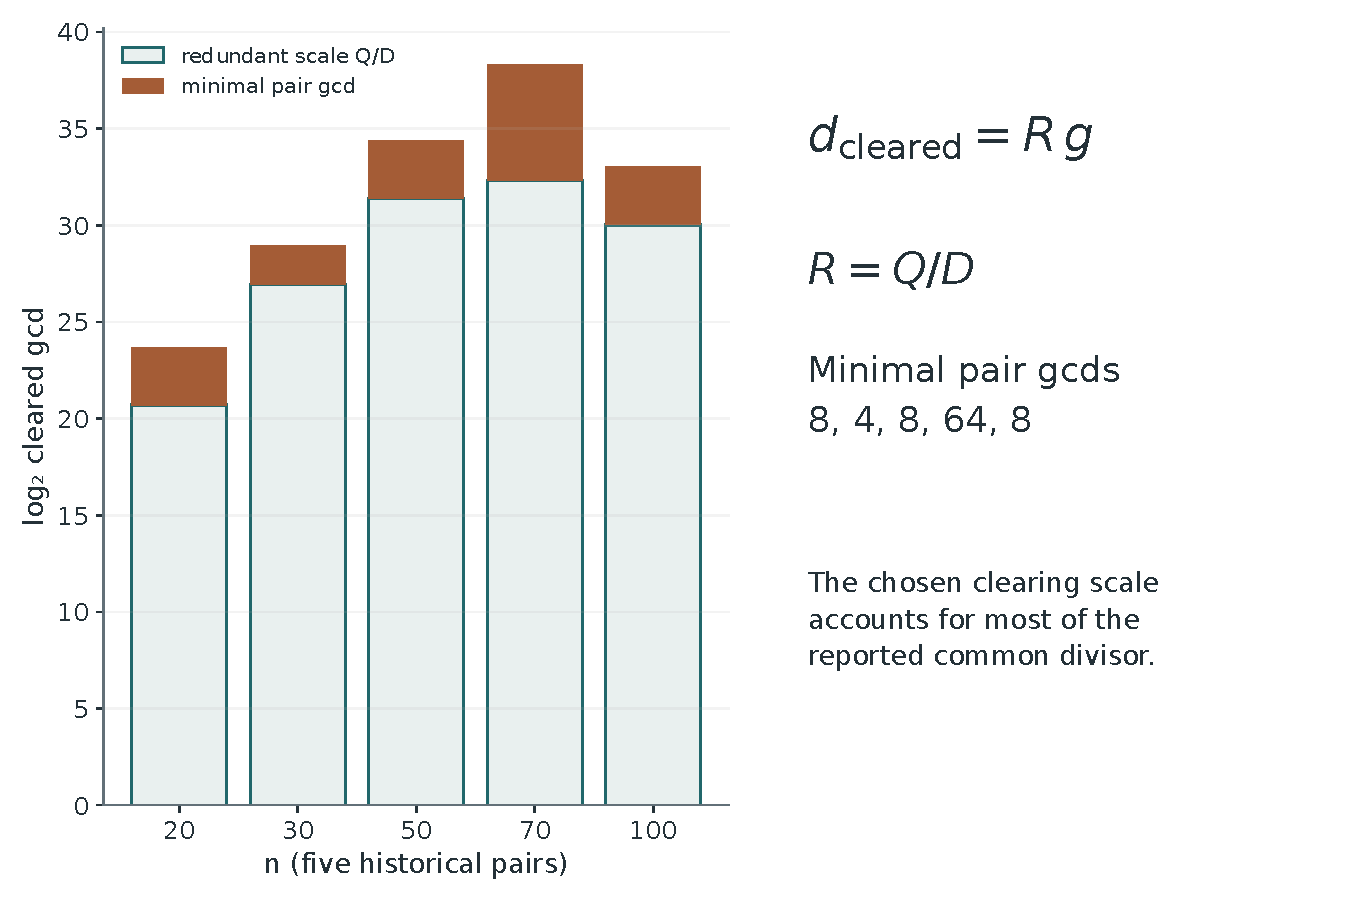
\includegraphics[width=0.96\linewidth]{../visual/figures/24_gcd_decomposition.pdf}
\caption{The cleared gcd splits into redundant scale and content of the minimally cleared pair. Each displayed bar belongs to one of the five exact computations.}
\label{fig:content-decomposition}
\end{figure}

The distinction also affects the dyadic interpretation. At $(20,66)$, $v_2(h)=3$, while $v_2(g)=20$. The remaining seventeen powers of $2$ occur in $Q/D$. At $(70,232)$, the corresponding split is $6+21=27$. A plotted valuation of the cleared gcd does not by itself measure the dyadic content of the packet.

\section{Rates are observations until quantified}

The historical display divides $\log g$ by $n+m$. Its five values decrease from approximately $0.19102$ to $0.05297$. These are useful diagnostics of the sampled pairs. They do not prove $\log g=o(n+m)$, a monotonicity theorem, or a bound at every subsequent pair. Even the sampling rule matters. A result along one sequence $m=m(n)$ is weaker than a bound uniform over a two dimensional range of indices.

\begin{figure}[htbp]
\centering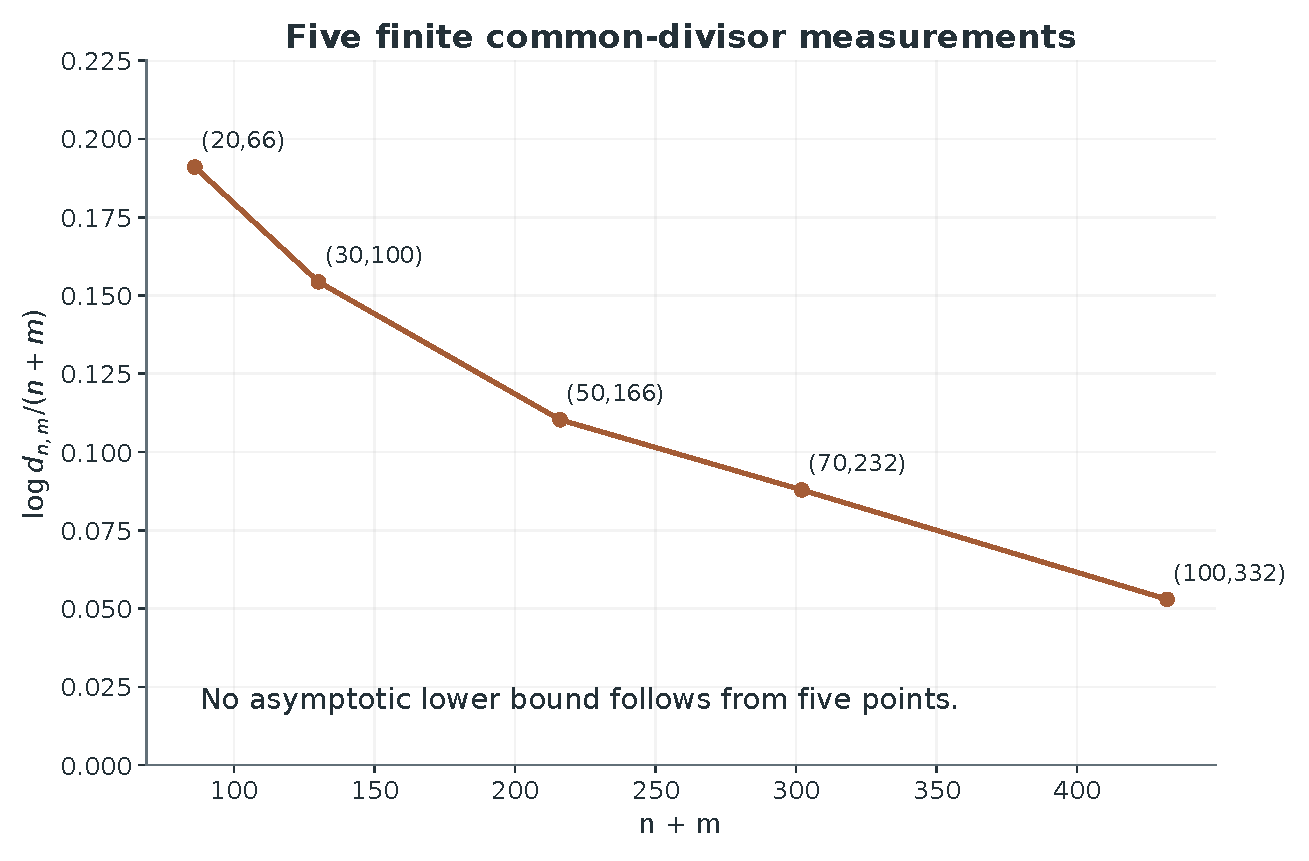
\includegraphics[width=0.96\linewidth]{../visual/figures/23_gcd_rate.pdf}
\caption{The historical logarithmic ratios decrease at the five sampled pairs. The line joins observations and carries no prediction beyond them.}
\label{fig:sampled-content-rate}
\end{figure}

The exact decomposition yields a more informative identity for rate analysis:
\begin{equation}
 \log g=\log Q-\log D+\log h.
 \label{eq:log-content-split}
\end{equation}
Suppose a future proof supplies limits for the three terms on the right along a chosen family. Then \eqref{eq:log-content-split} determines the cleared content rate. At present, the five rows supply values, not those limits. The identity separates the questions that a proof would need to answer. How much smaller is the true packet denominator than the universal denominator? How large is primitive common content? Are the bounds valid along every index in the chosen family?

There is a further one-sided relation to the binomial valuation scan. Because $h\mid U$, one always has $v_2(h)\leq v_2(U)$. If a universal estimate $v_2(U)=o(n+m)$ were proved, it would force the dyadic part of $h$ to be subexponential. It would not control odd factors of $h$, nor the factor $Q/D$. Conversely, a large cleared dyadic gcd can coexist with small $v_2(U)$ because most of its dyadic factor may come from redundant clearance.

This is why neither the large Pascal scan nor the five cleared gcds close the irrationality argument. They examine related arithmetic features, but they do not yet provide a complete uniform estimate for the primitive linear forms. The next chapter states exactly what that estimate must accomplish.

\chapter{The asymptotic bottleneck}
\label{chap:asymptotic-bottleneck}

\section{A nonzero family with an explicit analytic bound}

An irrationality argument needs an infinite family, not simply many successful finite values. For the present filter, a convenient family chooses an even integer $m=m(n)$ with $m/n\to\alpha\geq0$. Evenness supplies nonvanishing by a written integral argument. The slope supplies a definite analytic scale.

Write
\begin{equation}
 \phi=\frac{1+\sqrt5}{2},\qquad t=\phi^{-5},
 \qquad R=16\phi^5=88+40\sqrt5.
 \label{eq:asymptotic-constants}
\end{equation}
The unfiltered integral has the representation
\begin{equation}
 J_k=\int_{[0,1]^2}\psi(x,y)^k\,\dd\mu(x,y),
 \quad
 \psi=\frac{xy(1-x)(1-y)}{1-xy},
 \quad
 \dd\mu=\frac{\dd x\,\dd y}{\sqrt{x(1-y)}(1-xy)}.
 \label{eq:bottleneck-measure}
\end{equation}
The measure has finite total mass $J_0=8G$. The factor $1-xy$ in its denominator lies outside the square root. Moving it inside changes the integral and invalidates the coefficient identification.

Expanding the filter gives
\begin{equation}
 \widetilde J_{n,m}
 =\int_{[0,1]^2}\psi^n(1-16\psi)^m\,\dd\mu.
 \label{eq:bottleneck-filter}
\end{equation}
The range of $\psi$ is contained in $[0,t]$ and reaches its positive maximum $t$. In particular $t>1/16$. The filter factor therefore changes sign within the integration region. When $m$ is even, the integrand is nonnegative. It is strictly positive on an open subset of the interior on which $\psi>0$ and $\psi\ne1/16$. The density of $\mu$ is positive there. Hence
\begin{equation}
 \widetilde J_{n,m}>0\qquad(m\ \text{even}).
 \label{eq:even-filter-positive}
\end{equation}
This is a universal nonvanishing result. It uses neither a decimal value of $G$ nor a finite sign scan. For odd $m$, the same proof does not apply.

\section{Where the two branches of $M$ come from}

For $\alpha\geq0$, define
\begin{equation}
 M(\alpha)=\max\left\{
 \frac{1}{16(1+\alpha)}
 \left(\frac\alpha{1+\alpha}\right)^\alpha,
 \ t(16t-1)^\alpha
 \right\}.
 \label{eq:M-alpha}
\end{equation}
At $\alpha=0$ the first expression is assigned its continuous value $1/16$. This avoids treating the displayed $0^0$ as an algebraic input. The formula is Eskandari's source bound, with the recurrence normalization translated explicitly in LC06 and LC07~\cite{Eskandari2026}.

It can also be understood directly from the filter. On $0\leq s\leq1/16$, maximize $s(1-16s)^\alpha$. For $\alpha>0$, logarithmic differentiation gives
\begin{equation*}
 \frac1s-\frac{16\alpha}{1-16s}=0,
 \qquad s=\frac{1}{16(1+\alpha)}.
\end{equation*}
Substituting this point gives the first branch in \eqref{eq:M-alpha}. The endpoints give zero for $\alpha>0$, so this critical point is the maximum. At $\alpha=0$, the maximum on the interval is its right endpoint $1/16$.

On $1/16\leq s\leq t$, maximize $s(16s-1)^\alpha$. For $\alpha>0$ its logarithmic derivative is
\begin{equation*}
 \frac1s+\frac{16\alpha}{16s-1}>0.
\end{equation*}
Its maximum is therefore $t(16t-1)^\alpha$. The same conclusion holds at $\alpha=0$ because the function is then $s$. These two regions explain both branches and the need to retain their maximum.

Let $\alpha_n=m(n)/n$. The finite measure in \eqref{eq:bottleneck-filter} gives
\begin{equation}
 |\widetilde J_{n,m(n)}|
 \leq 8G\,M(\alpha_n)^n.
 \label{eq:actual-M-bound}
\end{equation}
Continuity of the two branches, including their stated extension at zero, then proves
\begin{equation}
 \limsup_{n\to\infty}
 |\widetilde J_{n,m(n)}|^{1/n}\leq M(\alpha).
 \label{eq:M-limsup}
\end{equation}
This is an upper bound. An equality for the actual integral would require a further argument. In particular, an upper bound does not measure the effect of sign cancellation in an odd filter.

\section{The external denominator scale}

The prime number theorem supplies the standard asymptotic~\cite{Zagier1997}
\begin{equation}
 \log L_k=k+o(k).
 \label{eq:PNT-LCM}
\end{equation}
Indeed $\log L_k=\sum_{p^a\leq k}\log p$ is the Chebyshev function $\psi_{\rm Ch}(k)$, and its ratio to $k$ tends to one. Source contract LC10 records the prime number theorem and the elementary prime power conversion. Equivalently, write $\log L_k=\sum_{a\geq1}\vartheta(k^{1/a})$, where $\vartheta(x)=\sum_{p\leq x}\log p$. The first term is $k+o(k)$. The remaining terms are $O(\sqrt{k}\log k)=o(k)$, using $\vartheta(x)=O(x)$ and at most $\log_2 k$ nonzero terms. The symbol $\psi_{\rm Ch}$ here denotes the arithmetic function, not the two variable kernel in \eqref{eq:bottleneck-measure}. The prime number theorem is an external theorem. The finite lcm calculations in this publication do not reprove it.

Set
\begin{equation}
 K_n=16^nL_{2(n+m(n))}^2.
 \label{eq:K-asymptotic}
\end{equation}
For $m(n)/n\to\alpha$, \eqref{eq:PNT-LCM} gives
\begin{equation}
 \frac{\log K_n}{n}\longrightarrow
 \kappa_0(\alpha)=\log16+4(1+\alpha).
 \label{eq:kappa-alpha}
\end{equation}
The factor $4$ has a precise origin. The lcm index is $2(n+m)$, and the lcm is squared. Missing either factor would create an incorrect apparent decay margin. The subscript in $\kappa_0$ emphasizes that this is the clearing cost alone. Define the combined bound exponent by $E(\alpha)=\kappa_0(\alpha)+\log M(\alpha)$.

With the cleared gcd $g_n=g_{n,m(n)}$, the primitive form is exactly
\begin{equation}
 \Lambda_n=\frac{K_n}{g_n}\widetilde J_{n,m(n)}.
 \label{eq:Lambda-bottleneck}
\end{equation}
Suppose a future arithmetic argument establishes
\begin{equation}
 \delta=\liminf_{n\to\infty}\frac{\log g_n}{n}.
 \label{eq:delta-content}
\end{equation}
For finite $\delta$, the present analytic estimate yields
\begin{equation}
 \limsup_{n\to\infty}\frac{\log|\Lambda_n|}{n}
 \leq\kappa_0(\alpha)+\log M(\alpha)-\delta.
 \label{eq:margin-inequality}
\end{equation}
The same interpretation applies when $\delta=+\infty$: any sufficiently large finite lower bound for the content rate would suffice. All logarithms of nonzero forms are legitimate for the even family by \eqref{eq:even-filter-positive}. The strict negativity of the right side is the missing sufficient margin. A zero margin would not suffice, because lower order terms could still prevent convergence to zero.

\section{What the current bound fails to supply}

Even without numerical optimization, the explicit bound reveals a limitation. Its cleared exponent before content reduction is positive for every slope.

\begin{proposition}[The displayed upper bound has no cleared decay margin]
\label{prop:positive-cleared-upper}
For every $\alpha\geq0$,
\begin{equation}
 \kappa_0(\alpha)+\log M(\alpha)>0.
 \label{eq:positive-bound-rate}
\end{equation}
This statement concerns the exponent of the available upper bound. It is not a lower bound on the actual primitive forms.
\end{proposition}

\begin{proof}
Put $c=16t-1$. The second branch in \eqref{eq:M-alpha} gives
\begin{equation*}
 \kappa_0(\alpha)+\log M(\alpha)
 \geq 4+\log(16t)+\alpha(4+\log c).
\end{equation*}
Now $t=(5\sqrt5-11)/2>5/64$. For example, this inequality follows by squaring the positive rational bound $\sqrt5>357/160$, since $5\cdot160^2>357^2$. Thus $16t>5/4>1$ and $c>1/4$. Consequently the last display is greater than $4+\alpha(4-\log4)>0$.
\end{proof}

The proposition says that the direct combination of $M$ with the chosen denominator bound does not prove shrinking integer forms without a quantified content gain. It does not say that the actual forms diverge. A growing upper bound is compatible with a quantity that decays rapidly. Stronger analytic estimates or smaller actual denominators can change the conclusion, but each requires its own proof.

At the source's approximately optimal slope $\alpha=3.31765$, the two branches of $M$ are near $0.006040$. The resulting exponent $\kappa_0+\log M$ is about $14.93384$ per unit $n$. These are rounded evaluations of explicit formulas, not certified extrema or an estimate for $\log|\Lambda_n|/n$. They show how large a content rate would need to be for this particular upper bound to force decay. The five observed gcd ratios are reported per $n+m$ and cannot be substituted as asymptotic rates in this calculation.

\begin{figure}[htbp]
\centering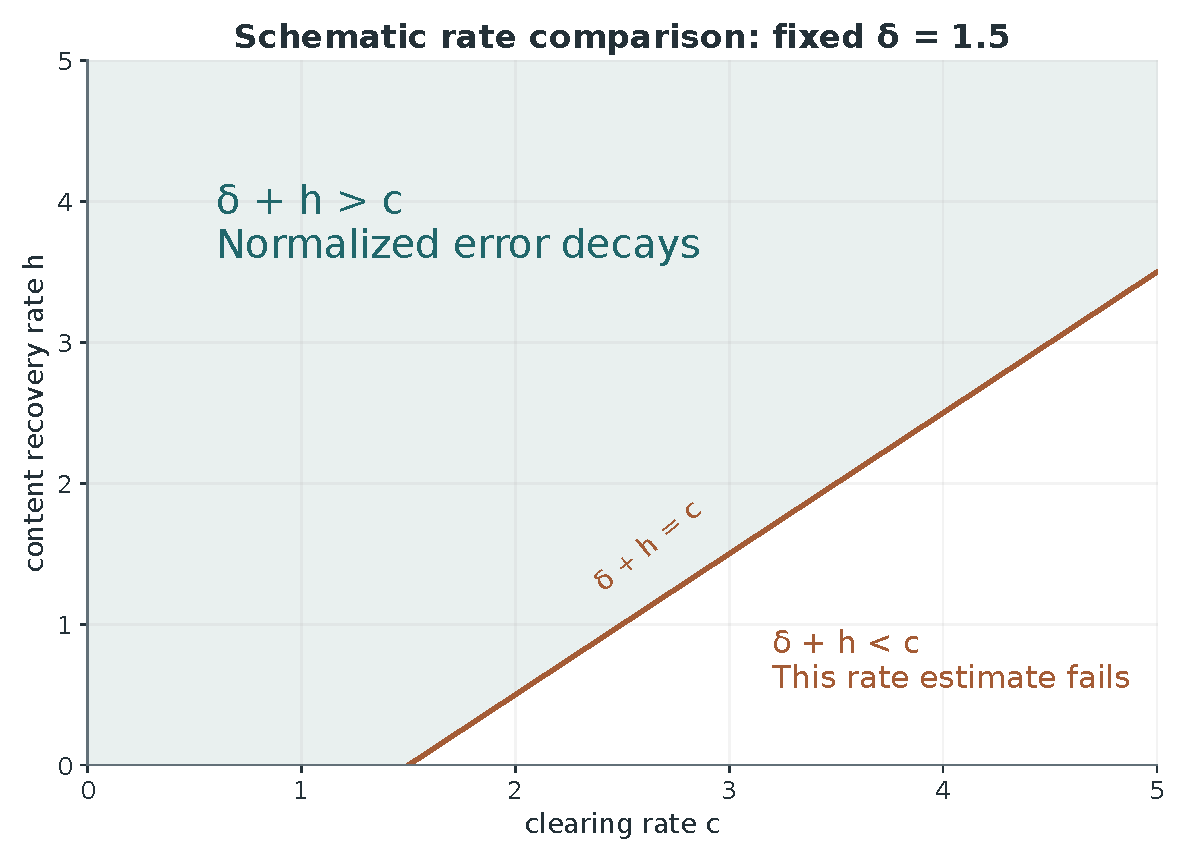
\includegraphics[width=0.96\linewidth]{../visual/figures/25_threshold_plane.pdf}
\caption{A strict negative margin is sufficient for decay after clearing and reduction. The boundary compares exponential rates. Finite measurements do not establish a point's asymptotic location.}
\label{fig:threshold-margin}
\end{figure}

\section{The source approximation exponent}

Eskandari's coefficient growth statement is
\begin{equation}
 \lim_{n\to\infty}\frac{\log|\widetilde U_{n,m(n)}|}{n}
 =\gamma(\alpha)
 =-\log16+\log R+\alpha\log(1+R),
 \label{eq:gamma-alpha}
\end{equation}
where $\widetilde U=8(-1)^n16^{-n}U$. This is an external asymptotic result in the preprint, not a conclusion of the finite recurrence audit. Together with the filter bound it controls the approximation error
\begin{equation}
 \left|G-\frac VU\right|
 =\frac{|\widetilde J|}{|\widetilde U|}.
 \label{eq:approximation-error}
\end{equation}
Before any additional quantified gcd saving, the reduced denominator $q$ is at most the absolute cleared coefficient $|A|$. Its available exponent is
\begin{equation}
 c_A(\alpha)=4(1+\alpha)+\log R+\alpha\log(1+R).
 \label{eq:cA-alpha}
\end{equation}
The source's resulting guaranteed approximation exponent is
\begin{equation}
 \eta(\alpha)=
 \frac{\log R+\alpha\log(1+R)-\log16-\log M(\alpha)}
 {4(1+\alpha)+\log R+\alpha\log(1+R)}.
 \label{eq:eta-alpha}
\end{equation}
The source reports a maximum near $0.62335$ at $\alpha\approx3.31765$ and states its theorem in the rounded form $\eta\geq0.62$~\cite{Eskandari2026}. The present edition records that as a preprint result with its stated dependencies. It does not upgrade it to a peer reviewed theorem, a certified global numerical maximum, or an irrationality proof.

The denominator index in \eqref{eq:eta-alpha} is $n$, while the filter depth grows like $\alpha n$. This is why the lcm term is $4(1+\alpha)$ rather than $4$. Replacing $n$ by $n+m$ consistently rescales every rate. Rescaling just one term changes the statement and is invalid.

An approximation exponent below one cannot contradict rationality. If $G=a/b$ were rational and $p/q\ne a/b$ were reduced, then
\begin{equation}
 \left|\frac ab-\frac pq\right|
 =\frac{|aq-bp|}{bq}\geq\frac1{bq}.
 \label{eq:rational-approx-lower}
\end{equation}
A bound of order $q^{-0.62}$ is larger than this obstruction for large $q$. Even rational numbers have many distinct approximations of that quality. For example $a/b+1/(bk)$ has error $1/(bk)$ and, after reduction, denominator at most $bk$. Nothing in such a bound isolates irrationality.

The identity $c_A-\gamma=\kappa_0$ gives another way to read the threshold. The unreduced exponent satisfies $\eta>1$ exactly when $\kappa_0+\log M<0$. Proposition~\ref{prop:positive-cleared-upper} shows why the displayed source estimate does not reach that regime. A genuine content saving changes the denominator and the primitive error together. It cannot be inserted in just one side of the comparison.

\section{A precise conditional completion theorem}

\begin{theorem}[Sufficient content margin]
\label{thm:conditional-completion}
Choose even integers $m(n)\geq0$ such that $m(n)/n\to\alpha\geq0$. Use the coefficient clearing theorem, the corrected filter identity, and the prime number theorem as specified above. If there exists a real number $\delta_0$ with
\begin{equation}
 \liminf_{n\to\infty}\frac{\log g_{n,m(n)}}{n}\geq\delta_0
 \quad\text{and}\quad
 \delta_0>\kappa_0(\alpha)+\log M(\alpha),
 \label{eq:conditional-content-hypothesis}
\end{equation}
then $G$ is irrational.
\end{theorem}

\begin{proof}
The coefficient clearing theorem and division by the exact gcd make $\Lambda_n=a_nG-b_n$ with $a_n,b_n\in\Z$. Evenness of $m(n)$ makes $\widetilde J_{n,m(n)}>0$, so \eqref{eq:Lambda-bottleneck} gives $\Lambda_n>0$. Choose $\varepsilon>0$ so that $3\varepsilon<\delta_0-\kappa_0(\alpha)-\log M(\alpha)$. For all sufficiently large $n$, the clearing asymptotic gives $K_n\leq\exp((\kappa_0+\varepsilon)n)$, the filter bound gives $|\widetilde J_{n,m(n)}|\leq\exp((\log M+\varepsilon)n)$, and the liminf assumption gives $g_{n,m(n)}\geq\exp((\delta_0-\varepsilon)n)$. Therefore
\begin{equation*}
 0<\Lambda_n\leq
 \exp\bigl((\kappa_0+\log M-\delta_0+3\varepsilon)n\bigr)
 \longrightarrow0.
\end{equation*}
If $G=a/b$ with integers $a,b$ and $b>0$, then $b\Lambda_n=aa_n-bb_n$ is a positive integer. It is at least one, so $\Lambda_n\geq1/b$. This contradicts the displayed convergence.
\end{proof}

The proof of this implication is complete. Its content hypothesis is not established here. The theorem is therefore conditional, and cannot be listed as a proof of the conjecture. It supplies a concrete target for a future arithmetic result. A stronger analytic bound could replace $M$, provided it were proved for the same infinite family and retained the nonvanishing input.

There is also a formulation independent of the universal clearing choice. With $D_n,h_n$ as in Chapter~\ref{chap:primitive-content}, the primitive error is $(-1)^n(D_n/h_n)(S_{n,m(n)}G-H_{n,m(n)})$. An estimate directly on that expression would suffice. If denominator reduction yields a provably smaller exponential cost, the excess factor $Q_n/D_n$ should simply be removed from the accounting. The irrationality criterion itself is unchanged.

\begin{figure}[htbp]
\centering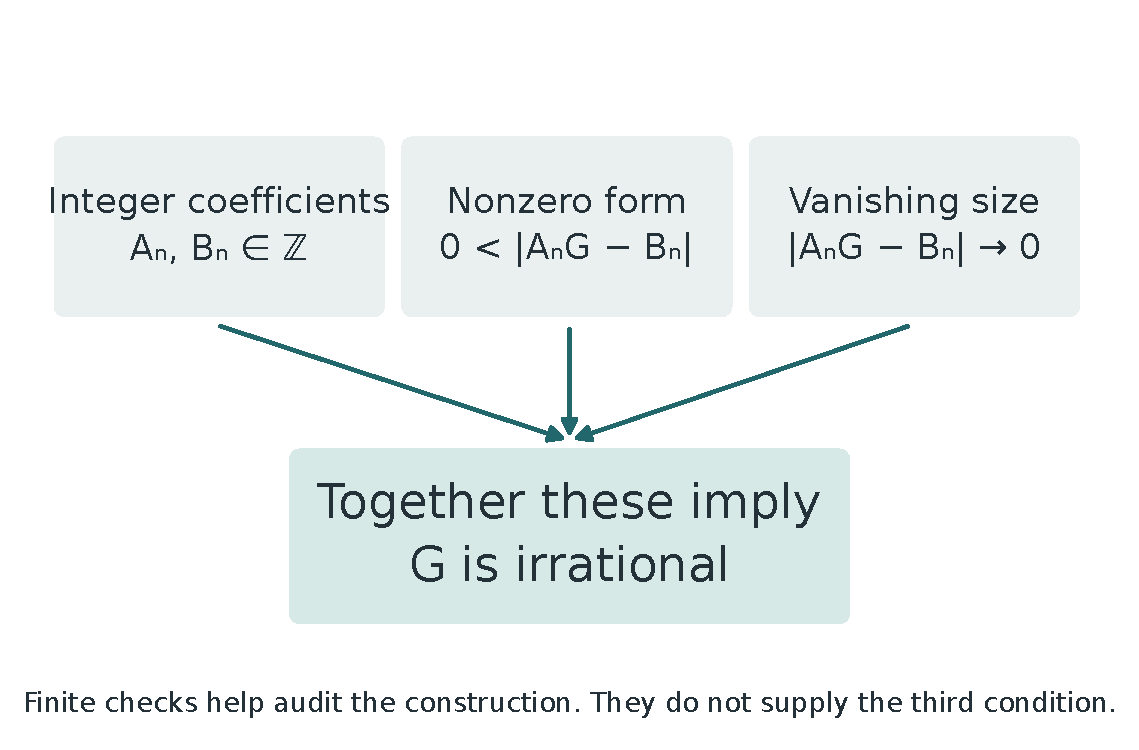
\includegraphics[width=0.96\linewidth]{../visual/figures/28_conditional_route.pdf}
\caption{The conditional route separates integer coefficients, nonvanishing, and a strict decay margin. The first two have stated source or written proofs here. The final global estimate remains open.}
\label{fig:conditional-route}
\end{figure}

\section{Why a finite prefix cannot supply the final hypothesis}

There is a simple logical reason to resist extrapolation. Given any finite list of positive values $x_1,\ldots,x_N$, it has a positive extension that tends to zero and another positive extension that tends to infinity. Keep the list fixed and set the tail to $e^{-n}$ in the first case or $e^n$ in the second. Similarly, any finite list of positive integer gcds can be extended by $1$ forever or by integers with an arbitrarily prescribed positive exponential rate.

These extensions are not asserted to satisfy the Catalan recurrence. They illustrate a narrower point: finite values by themselves do not imply an asymptotic property. The recurrence, integral, or arithmetic structure must supply the bridge. A theorem using that structure could settle a uniform estimate. The prefix alone cannot.

A positive exponent in an upper bound has the same logical limitation. If $x_n\leq e^{cn}$ with $c>0$, both $x_n=e^{-n}$ and $x_n=e^{cn/2}$ satisfy the bound eventually. One sequence decays and the other grows. Thus the failure of the bound to force decay is a proved limitation of the estimate, not proof of divergence of the object it bounds.

\begin{figure}[htbp]
\centering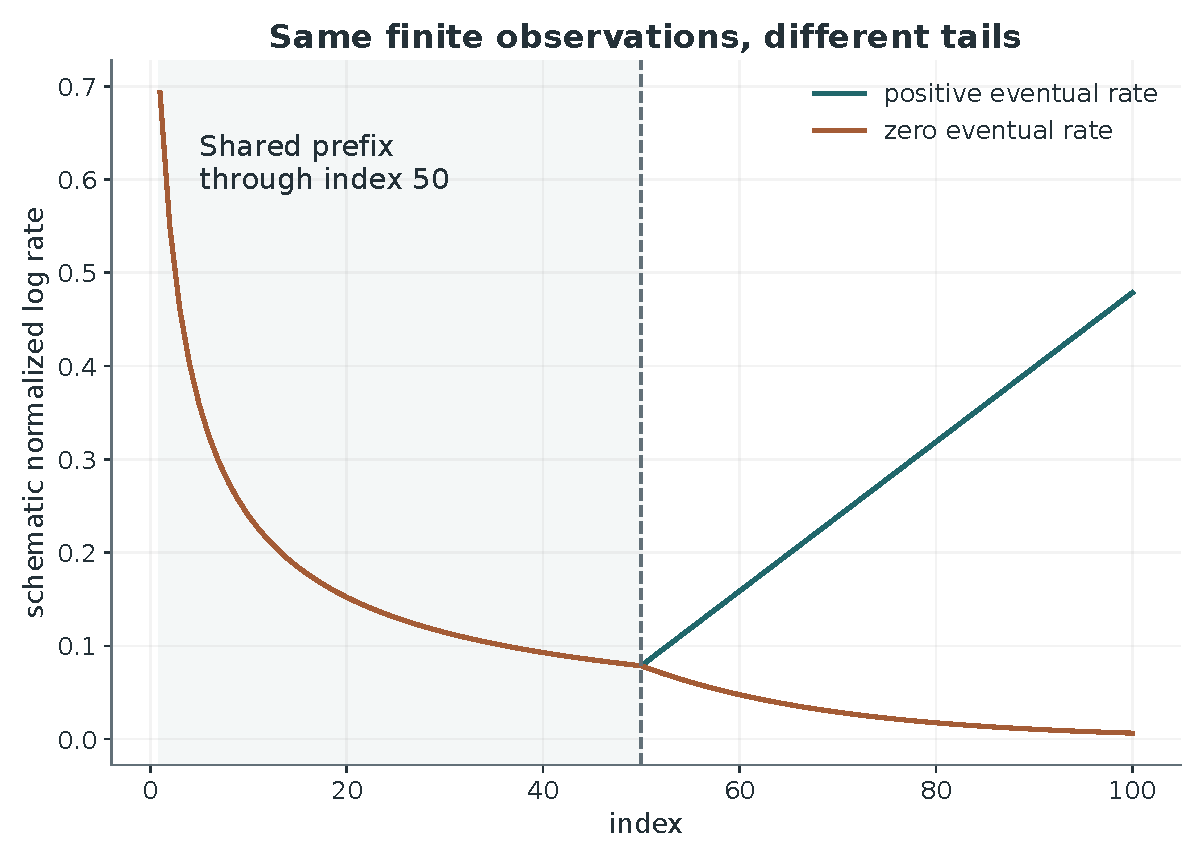
\includegraphics[width=0.96\linewidth]{../visual/figures/26_finite_countermodels.pdf}
\caption{Finite data can agree with incompatible asymptotic extensions. The illustrated tails are logical examples, not alternative Catalan recurrences.}
\label{fig:finite-countermodels}
\end{figure}

The same caution applies to the modular scan. Its $8\,006\,000$ exact valuations establish a large finite statement. They do not prove $v_2(S_{n,m})=o(n+m)$ outside the scanned domain, a uniform bound on odd common factors, or the lower bound on $\log g$ in Theorem~\ref{thm:conditional-completion}. The achievement is reproducible bounded evidence and a sharply stated remaining implication.

\chapter{Evidence, status, and the next theorem}
\label{chap:evidence-status}

\section{What this edition establishes}

This publication assembles three different kinds of mathematical evidence. Written arguments establish identities and implications for all indices under their stated hypotheses. Source contracts identify external theorems and the precise normalization used to apply them. Exact computations establish statements on bounded ranges. These kinds of evidence reinforce one another, but they have different scopes.

The universal arguments written in this edition include the elementary half-binomial denominator lemma, the Wronskian induction, the Pascal identity, the modular valuation criterion, the primitive content decomposition, and the conditional irrationality implication. Some of these arguments start from externally supplied identities. For example, the integrality proof for $T_n$ uses the authenticated half-binomial expression for $u_n$. Its universal arithmetic step is written here, while the identity identifying that expression with the recurrence is an external input.

The integral normalization receives special attention because the printed source contains a factor discrepancy. In the historical recurrence normalization, the correct relation is
\begin{equation}
 u_nG-v_n=\frac{(-1)^n}{8}J_n.
 \label{eq:status-normalization}
\end{equation}
The printed factor $1/4$ is incompatible with $u_0=1$ and the exact evaluation $J_0=8G$. The source audit also checks the all-index normalization through the displayed hypergeometric transformation and partial-fraction coefficient identification. This is an explicit correction with stated dependencies. It is not a silently altered quotation, nor a claim that a published erratum was recovered.

The same separation applies to asymptotic results. The recurrence's growth rates, its limit identification, strong coefficient clearing, and the prime number theorem are external inputs. The exact translation of those results and their combination into an irrationality criterion are written project arguments. No amount of finite recurrence agreement alone proves the externally supplied limit or denominator theorem.

\begin{table}[htbp]
\centering\small
\begin{tabularx}{\linewidth}{@{}p{0.29\linewidth}X@{}}
\toprule
Evidence class & Meaning in this edition\\
\midrule
Written universal argument & A proof applies to every index in its stated domain. External premises remain named.\\
External source input & An authenticated result is translated with its exact initial conditions, factors, and index range.\\
Finite exact computation & Integer or rational decisions are verified only at the recorded inputs.\\
Rounded diagnostic display & Decimal logarithms and plots illustrate exact data or formulas. Their last digits are not theorem inputs.\\
Open estimate & A uniform asymptotic statement is specified, but not established.\\
\bottomrule
\end{tabularx}
\caption{Evidence classes used throughout the publication. The classification concerns the claim, not the prestige of its format.}
\label{tab:evidence-classes}
\end{table}

\section{The finite record}

The historical default run is reproduced without editing the historical program. Its new result JSON is byte for byte identical to the recovered result JSON. This is a strong implementation check for the recorded defaults, not a universal arithmetic theorem.

The large modular scan covers $1\leq n\leq2000$ and $0\leq m\leq4n$, a total of $8\,006\,000$ pairs. It finds maximum valuation $31$, with a witness at $(1466,2113)$ in the historical traversal order. No residue is zero modulo $2^{128}$, so every scanned valuation is below the precision ceiling and is exact. The direct witness calculation reconstructs the full integer sum and verifies the same valuation. The evidence does not assert that this maximizing pair is unique.

The smaller direct grid contains $20\,300$ pairs with $n\leq100$. It agrees with the modular Pascal computation at every pair and has maximum valuation $20$ at $(52,6)$ in its own traversal order. A deliberate low precision test at modulus $2^4$ produces eight zero residues in the much smaller domain $n\leq3$. These are correctly marked unresolved. The true direct maximum there is $6$, while the clipped residue report is $4$. This negative control checks that the program does not mistake a precision ceiling for an exact valuation.

Independent rational recurrence calculations agree through $n=500$. The integer recurrence for $T_n$ has zero remainder at every division through $n=10000$. The half-binomial check verifies all $1\,326$ summands through $n=50$. These finite checks support the implementation and normalization. Their universal counterparts still depend on the written arguments and external coefficient identity.

The five gcd computations in Chapter~\ref{chap:primitive-content} are exact rational calculations, including complete numerator and denominator strings. The displays of $\log g/(n+m)$ are ordinary rounded logarithms. The exact factorization and decomposition are the arithmetic evidence. The display ratios are explanatory summaries.

\section{The failed sign guess remains part of the record}

A diagnostic guess proposed during this audit asserted $\operatorname{sign}F_{n,m}=(-1)^m$ for the raw packet form
\begin{equation}
 F_{n,m}=8(-1)^n\bigl(S_{n,m}G-H_{n,m}\bigr).
 \label{eq:status-raw-F}
\end{equation}
It fails. Already at $(n,m)=(1,1)$,
\begin{equation}
 F_{1,1}=\frac{173056}{9}-20992G>0,
 \label{eq:status-sign-counterexample}
\end{equation}
while the guess predicts a negative sign. A certified rational interval for $G$ determines the sign. Among the $860$ tested pairs with $1\leq n\leq20$ and $0\leq m\leq4n$, there are $138$ mismatches with the guess. All $860$ actual forms are nevertheless certified nonzero.

The failed guess was an exploratory diagnostic of this audit. It was not an authenticated source theorem. Its failure does not contradict the even-filter positivity proof, which has a different hypothesis and a direct integral justification. It does show why a proposed odd-filter sign rule cannot be carried into a global proof on the strength of a suggestive pattern.

The initial independent run retained every mismatch but gave the sign experiment an overly broad interpretive label. The corrected source and final rerun explicitly record falsification. Both runs are preserved. The publication uses the final interpretation and does not conceal the earlier label. The evidence report identifies the final independent directory as the current record.

\section{A dated statement about recent claims}

The edition date matters because recent primary preprints discuss the irrationality of $G$. Zhi-Wei Sun's preprint, submitted on 3 September 2026, claims a proof~\cite{Sun2026}. The checked arXiv history contained only version 1 on 9 October 2026. A subsequent note by Dane Wachs, submitted on 16 September and dated 15 September internally, identifies a gap in a displayed asymptotic derivation~\cite{Wachs2026}. It describes a quadratic contribution from the prime $2$ that it says the derivation does not account for.

These are attributed statements about the checked sources. This publication does not independently reproduce the determinant computations in the critical note. It does not treat that note as a universal theorem excluding every repair, nor import the claimed irrationality theorem from the first preprint. Neither source is described here as peer reviewed.

As of 9 October 2026, no proof of the irrationality of Catalan's constant is established by the material checked for this publication. A primary preprint claims a proof, and a subsequent primary note identifies an incomplete derivation. This edition does not resolve that dispute. A later verified result would require updating this dated status statement.

The source search is bounded. It checked the listed arXiv identifiers, relevant journal and author pages, the recurrence and denominator papers, and the filter preprint. It is not an exhaustive historical survey or a global novelty certification. Where a result is standard or already appears in a source, the edition says so. The filter is attributed to Eskandari. The recurrence and its asymptotic identification are attributed to Zudilin. The strong arithmetic theorem is attributed to Krattenthaler and Rivoal.

\section{What was recovered and what was reconstructed}

The historical project material recovered for this piece consists of the packet audit script, its result JSON, and its run log. Those files are preserved byte for byte. They establish a genuine earlier computational record. They do not contain a recovered monograph, a complete universal proof of irrationality, or a compiled Lean development.

The exposition in this edition is newly reconstructed around that record. It supplies mathematical context, explicit normalization checks, written arithmetic arguments, independent finite checks, source contracts, and a precise remaining asymptotic implication. This reconstruction is part of the publication work. It must not be backdated or presented as prose recovered from the original research session.

The companion source bundle contains the publication source, figure programs, public computation programs, exact outputs, and audit records. Primary papers are cited and their relevant contracts are documented. Complete downloaded third-party papers are not included in the public bundle. There is no Lean compiler certificate for this Catalan piece, because no such formalization was recovered or built for it. A written proof and a successful Python run are reported in their own categories.

\section{The next theorem has a precise shape}

The remaining target is not the vague instruction to find more cancellation. One possible completion is Theorem~\ref{thm:conditional-completion}: choose a specified even family, establish a uniform content rate, and prove a strict negative primitive error margin. Another possibility is a stronger analytic estimate that yields the same integer-form decay after the actual denominator cost is included. A third is a smaller denominator theorem for the filtered coefficients. Each route must retain the exact coefficient normalization and nonvanishing input.

The work can therefore be advanced in distinct, testable directions. An arithmetic route should distinguish $Q/D$ from $h$ and control both dyadic and odd factors where necessary. An analytic route should prove a bound for the actual integral along an infinite family, rather than infer decay from a plot. A formal route should encode the exact statements and mark external asymptotic inputs explicitly. More computation can expose candidates or counterexamples, but it must continue to state its range.

This edition is ready as an audited research account. Its identities, finite record, external dependencies, and open estimates are separated closely enough that a later result can be inserted at a definite point. The irrationality conclusion is not one of its established claims.


